\documentclass{article}

\usepackage[utf8]{inputenc}
\usepackage[brazil]{babel}

\title{Exercício 2: Perceptron Multicamadas}
\author{Rúbia Reis Guerra \\ 2013031143}

\usepackage{Sweave}
\begin{document}
\Sconcordance{concordance:MLP.tex:MLP.rnw:%
1 8 1 1 0 11 1 1 2 1 0 1 1 1 3 2 0 1 6 4 0 1 1 1 2 1 0 1 1 1 2 1 0 1 1 %
1 2 5 0 1 2 2 1 1 4 3 0 1 3 1 0 1 1 1 4 2 0 2 1 1 5 4 0 1 1 1 2 1 0 1 1 %
1 2 1 0 1 1 1 2 1 0 1 3 2 0 1 2 1 0 1 1 1 2 5 0 1 2 2 1 1 4 3 0 1 1 1 3 %
1 0 1 5 4 0 1 1 1 2 1 0 1 1 1 2 1 0 1 1 1 2 1 0 1 4 2 0 1 3 1 0 1 3 1 0 %
1 3 1 0 1 1 1 2 5 0 1 2 2 1 1 4 3 0 2 1 1 2 1 15 17 0 1 2 2 1 1 5 4 0 1 %
1 1 2 1 0 1 1 1 2 1 0 1 1 1 2 1 0 1 3 1 0 1 2 5 0 1 2 1 5 4 0 1 2 1 0 1 %
2 1 0 1 2 1 0 1 2 5 0 1 2 1 1}


\maketitle

\section{Multilayer Perceptron}
Um perceptron multicamada (MLP) é um modelo de rede neural artificial \textit{feedforward} que mapeia conjuntos de dados de entrada para um conjunto de saídas apropriadas. Um MLP consiste em várias camadas de nós em um grafo direcionado, com cada camada totalmente conectada à próxima. Exceto os nós de entrada, cada nó é um neurônio (ou elemento de processamento) com uma função de ativação não-linear. O MLP é uma modificação do perceptron linear e pode distinguir dados que não são linearmente separáveis. 
Nesta atividade, foi proposta a implementação de um MLP de duas camadas capaz de classificar um conjunto de pontos correspondente à função XOR.

\subsection{Implementação}
Inicialmente, criou-se o conjunto de pontos de entrada X = \{(0,0), (0,1), (1,0), (1,1)\}:

\begin{Schunk}
\begin{Sinput}
> library('plot3D')
> rm(list=ls())
> ################################################
> # Cria conjunto de pontos #
> X <- matrix(c(0,0,0,1,1,0,1,1), ncol = 2, byrow = T)
> ################################################
> # Plota pontos X[i,j] #
> plot(X[1,1], X[1,2], col='red', type='p', xlim=c(0,1),
+      ylim=c(0,1), xlab ='x_1', ylab='x_2',
+      sub='Figura 1: Conjunto de pontos (X)')
> par(new=T)
> plot(X[2,1], X[2,2], col='blue', type='p', xlim=c(0,1),
+      ylim=c(0,1), xlab='', ylab='')
> par(new=T)
> plot(X[3,1], X[3,2], col='blue', type='p', xlim=c(0,1),
+      ylim=c(0,1), xlab='', ylab='')
> par(new=T)
> plot(X[4,1], X[4,2], col='red', type='p', xlim=c(0,1),
+      ylim = c(0,1), xlab='', ylab='')
\end{Sinput}
\end{Schunk}
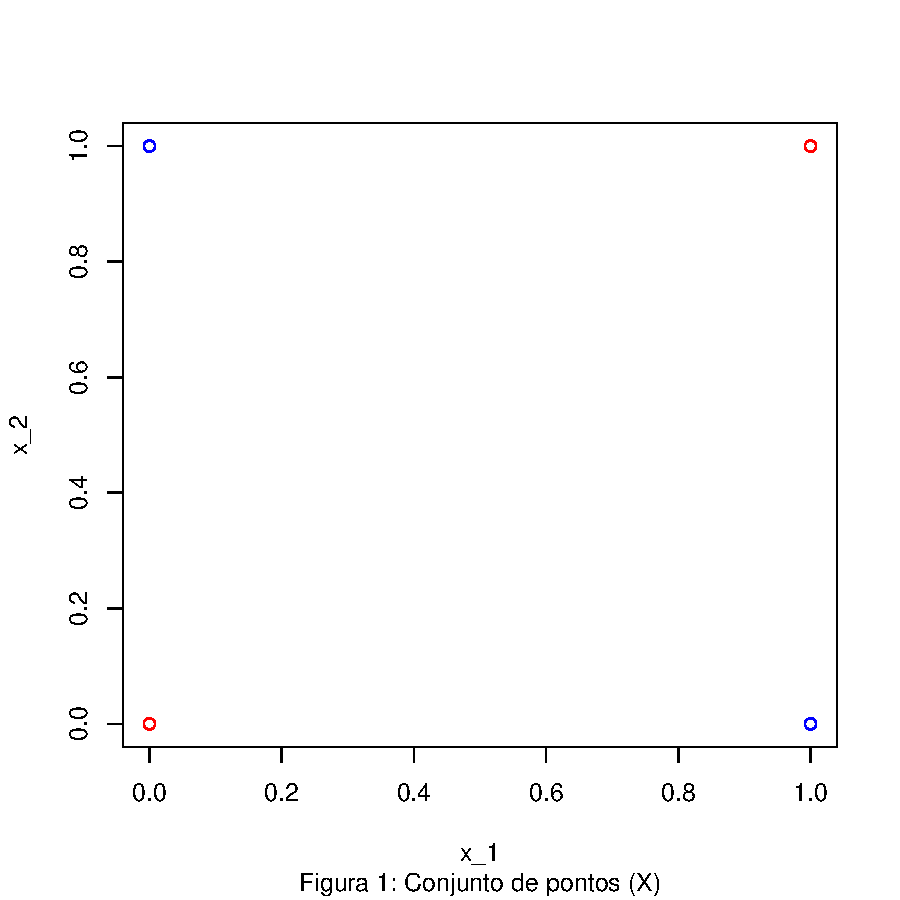
\includegraphics{MLP-001}

Em seguida, foram criados os vetores de pesos correspondentes aos separadores lineares de equações $x_{2} = -x_{1} - 1.5$ e $x_{2} = -x_{1} - 0.5$, equivalentes aos dois neurônios Perceptron da camada escondida (funções de ativação $h_{1}$ e $h_{2}$).

\begin{Schunk}
\begin{Sinput}
> ################################################
> # Adiciona unidades de bias #
> Xaug <- cbind(X,1)
> # Pesos da camada escondida #
> w1 <- matrix(c(1,1,-1.5), ncol = 1)
> w2 <- matrix(c(1,1,-0.5), ncol = 1)
> # Conjunto de pontos para gerar retas referentes 
> # às saídas dos neurônios da camada escondida #
> xt <- seq(0, 1, 0.1)
> y1 <- -xt + 1.5
> y2 <- -xt + 0.5
> ################################################
> # Plota pontos x[i,j] #
> plot(X[1,1],X[1,2], col='red', type='p', xlim=c(0,1),
+      ylim=c(0,1), xlab ='x_1', ylab='x_2',
+      sub='Figura 2: Separadores gerados na camada escondida')
> par(new=T)
> plot(X[2,1], X[2,2], col='blue', type='p', xlim=c(0,1),
+      ylim=c(0,1), xlab='', ylab='', sub='')
> par(new=T)
> plot(X[3,1], X[3,2], col='blue',type='p',xlim=c(0,1),
+      ylim=c(0,1), xlab='', ylab='', sub='')
> par(new=T)
> plot(X[4,1], X[4,2], col='red', type='p', xlim=c(0,1),
+      ylim=c(0,1), xlab='', ylab='', sub='')
> ################################################
> # Plot dos separadores gerados na camada escondida  #
> par(new=T)
> plot(xt, y1, col='red', type='l', xlim=c(0,1), 
+      ylim=c(0,1), xlab='', ylab='', sub='')
> par(new=T)
> plot(xt, y2, col='red', type='l', xlim=c(0,1),
+      ylim=c(0,1), xlab='', ylab='', sub='')
\end{Sinput}
\end{Schunk}
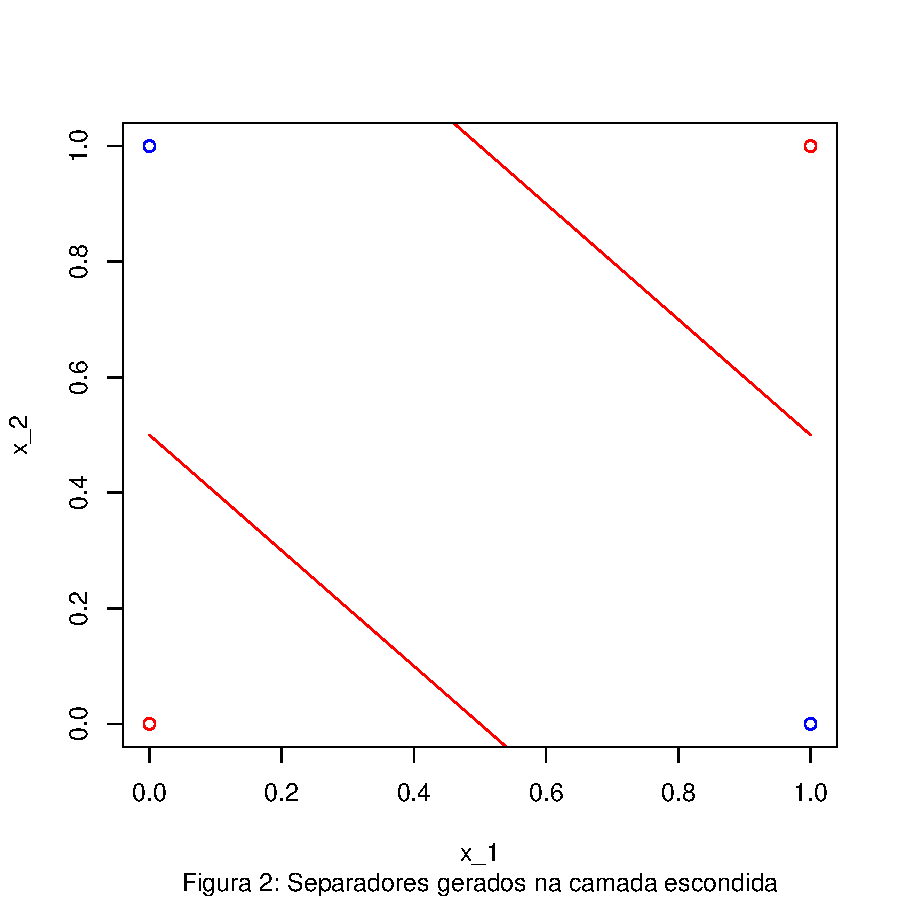
\includegraphics{MLP-002}

A partir das saídas geradas na camada escondida, foi obtida a matriz H, que corresponde ao conjunto de pontos \{(0,0), (0,1), (0,1), (1,1)\}. Em sequência, o conjunto de dados obtido foi fornecido à função de ativação da camada de saída $h_{3}$, gerando a reta com parâmetros correspondentes ao vetor de pesos $w_{3} = (0, -1, 0.5)$.

\begin{Schunk}
\begin{Sinput}
> ################################################
> # Funções de ativação da camada escondida #
> h1 <- 1*((Xaug %*% w1) >= 0)
> h2 <- 1*((Xaug %*% w2) >= 0)
> # Gera matriz h1, h2 #
> H <- cbind(h1, h2)
> ################################################
> # Plot dos resultados da camada escondida #
> plot(H[1,1], H[1,2], col='red', type='p', xlim=c(0,1), 
+      ylim=c(0,1), xlab='H_1', ylab='H_2',
+      sub='Figura 3: Resultados da camada escondida')
> par(new=T)
> plot(H[2,1], H[2,2], col='blue', type='p', xlim=c(0,1),
+      ylim=c(0,1), xlab='', ylab='', sub='')
> par(new=T)
> plot(H[3,1], H[3,2], col='blue', type='p', xlim=c(0,1),
+      ylim=c(0,1), xlab='', ylab='', sub='')
> par(new=T)
> plot(H[4,1], H[4,2], col='red', type='p', xlim=c(0,1),
+      ylim=c(0,1), xlab='', ylab='', sub='')
> ################################################
> # Pesos da camada de saída #
> w3 <- matrix(c(1,-1,0.5), ncol = 1)
> # Adiciona unidades de bias #
> Haug <- cbind(H, 1)
> # Funções de ativação da camada de saída #
> h3 <- 1*((Haug %*% w3) <= 0)
> # Plot do separador resultante da camada de saída #
> y3 <- xt + 0.5
> par(new=T)
> plot(xt, y3, col='red', type = 'l', xlim=c(0,1), 
+      ylim = c(0,1), xlab='', ylab='', sub='')
\end{Sinput}
\end{Schunk}
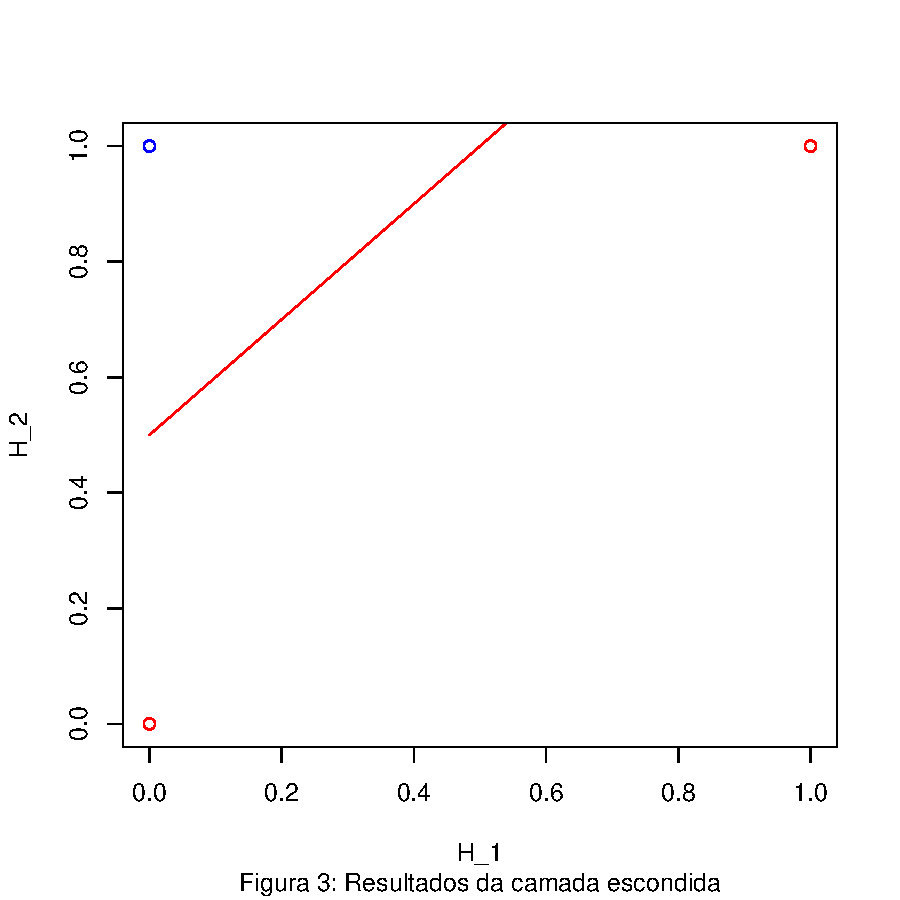
\includegraphics{MLP-003}

Enfim, aplicou-se a função perceptron no espaço $R^2$, gerando a superfície de separação esperada com base nos procedimentos anteriores.

\begin{Schunk}
\begin{Sinput}
> ################################################
> # Função Perceptron #
> seqi <- seq(0, 1, 0.05)
> seqj <- seq(0, 1, 0.05)
> M <- matrix(0, nrow =length(seqi), ncol=length(seqj))
> ci <- 0
> for(i in seqi)
+ {
+   cj <- 0
+   ci <- ci + 1
+   for (j in seqj)
+   {
+     cj <- cj + 1
+     xt <- c(i,j,1)
+     # Camada escondida #
+     h1 <- 1*((xt %*% w1) >= 0)
+     h2 <- 1*((xt %*% w2) >= 0)
+     # Camada de saída #
+     M[ci,cj] <- 1*((c(h1,h2,1) %*% w3) <= 0)
+   }
+ }
\end{Sinput}
\end{Schunk}

Gráficos obtidos:

\begin{Schunk}
\begin{Sinput}
> ################################################
> # Plota pontos x[i,j] #
> plot(X[1,1],X[1,2], col='red', type='p', xlim=c(0,1),
+      ylim=c(0,1), xlab ='x_1', ylab='x_2',sub='')
> par(new=T)
> plot(X[2,1], X[2,2], col='blue', type='p', xlim=c(0,1),
+      ylim=c(0,1), xlab='', ylab='', sub='')
> par(new=T)
> plot(X[3,1], X[3,2], col='blue',type='p',xlim=c(0,1),
+      ylim=c(0,1), xlab='', ylab='', sub='')
> par(new=T)
> plot(X[4,1], X[4,2], col='red', type='p', xlim=c(0,1),
+      ylim=c(0,1), xlab='', ylab='', sub='')
> # Plot da superfície de separação - 2D #
> par(new=T)
> contour(seqi, seqj, M,
+         sub='Figura 4: Superfície de separação - 2D')
\end{Sinput}
\end{Schunk}
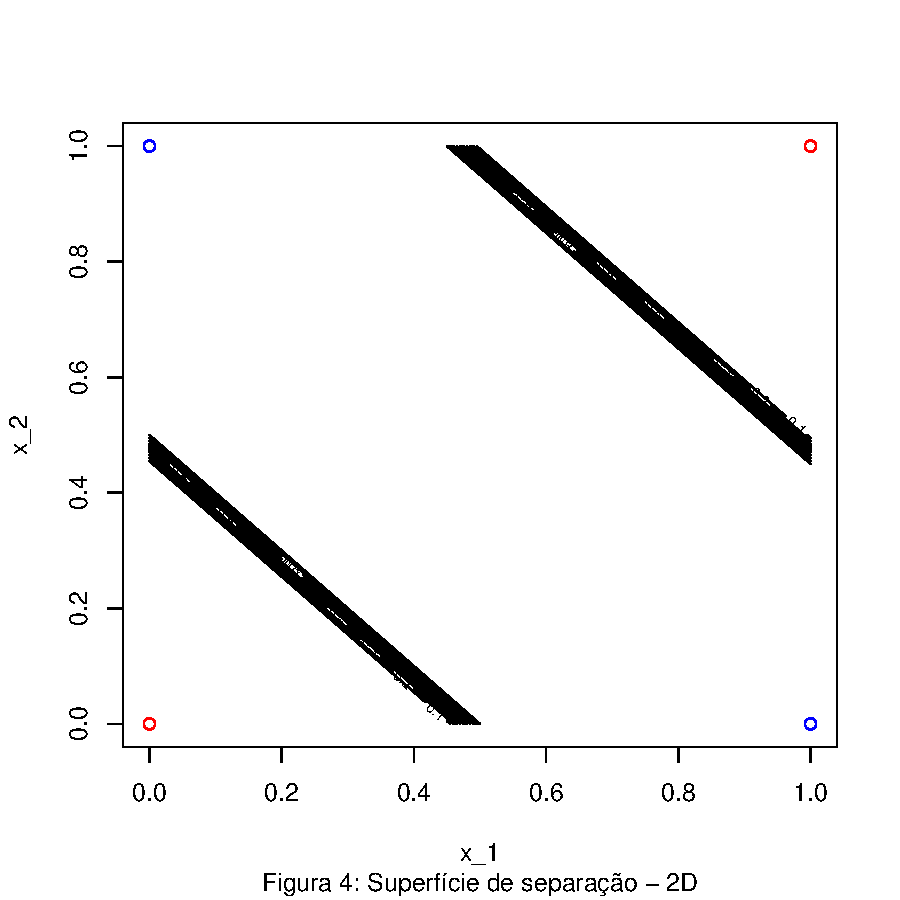
\includegraphics{MLP-005}

\begin{Schunk}
\begin{Sinput}
> ################################################
> # Plot da superfície de separação - 3D #
> persp3D(seqi, seqj, M, clim=c(0,2), contour=T,
+         sub='Figura 5: Superfície de separação - 3D')
> scatter3D(X[1,1], X[1,2], 1, col='red', type='p', 
+           xlim=c(0,1), ylim = c(0,1), add=T)
> scatter3D(X[2,1], X[2,2], 1, col='blue', type='p', 
+           xlim=c(0,1), ylim = c(0,1), add=T)
> scatter3D(X[3,1], X[3,2], 1, col='blue', type='p', 
+           xlim=c(0,1), ylim = c(0,1), add=T)
> scatter3D(X[4,1], X[4,2], 1, col='red', type='p', 
+           xlim=c(0,1), ylim = c(0,1), add=T)
\end{Sinput}
\end{Schunk}
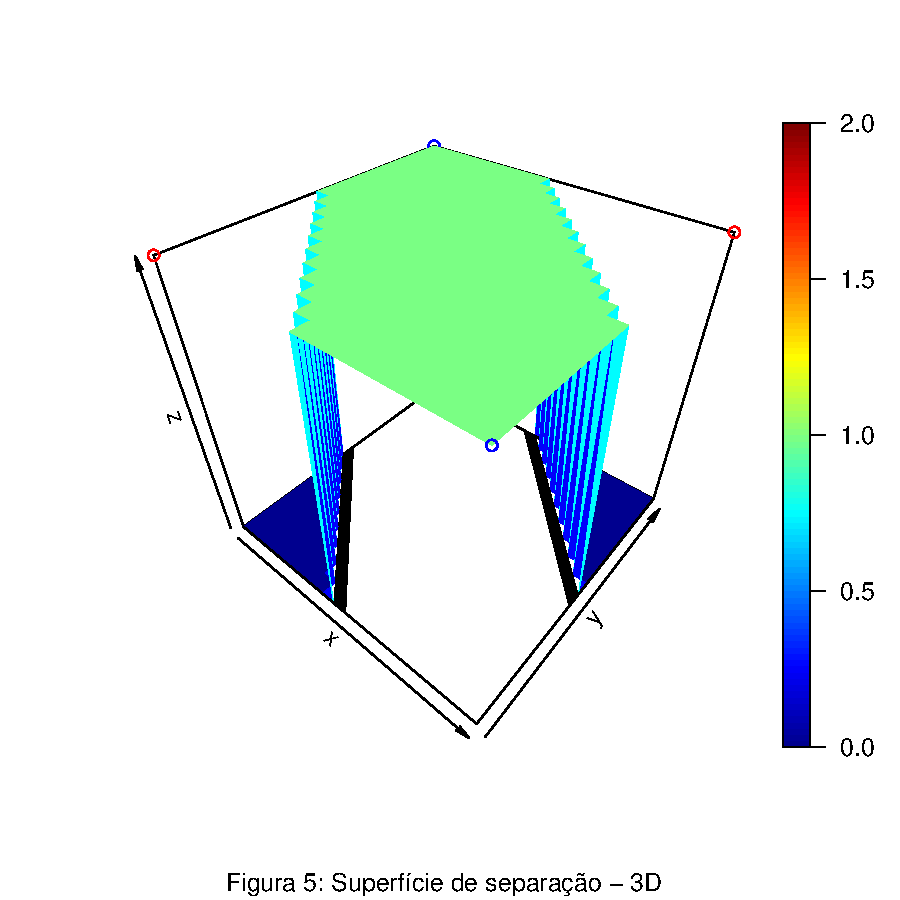
\includegraphics{MLP-006}

\end{document}
